\begin{quote} \textit{1) Estudiar las corrientes y tensiones en todos los componentes en función del tiempo, desde que se enciende el regulador ($t=0$) hasta régimen permanente. En particular, en régimen permanente, estudiar en detalle las corrientes y tensiones en un intervalo de unos pocos periodos.}
\end{quote}

%\HgraficarPNG{0.4}{fly}{Regulador \textit{Flyback} aislado.}{fig:cto}

\begin{figure}[H]
	\centering
	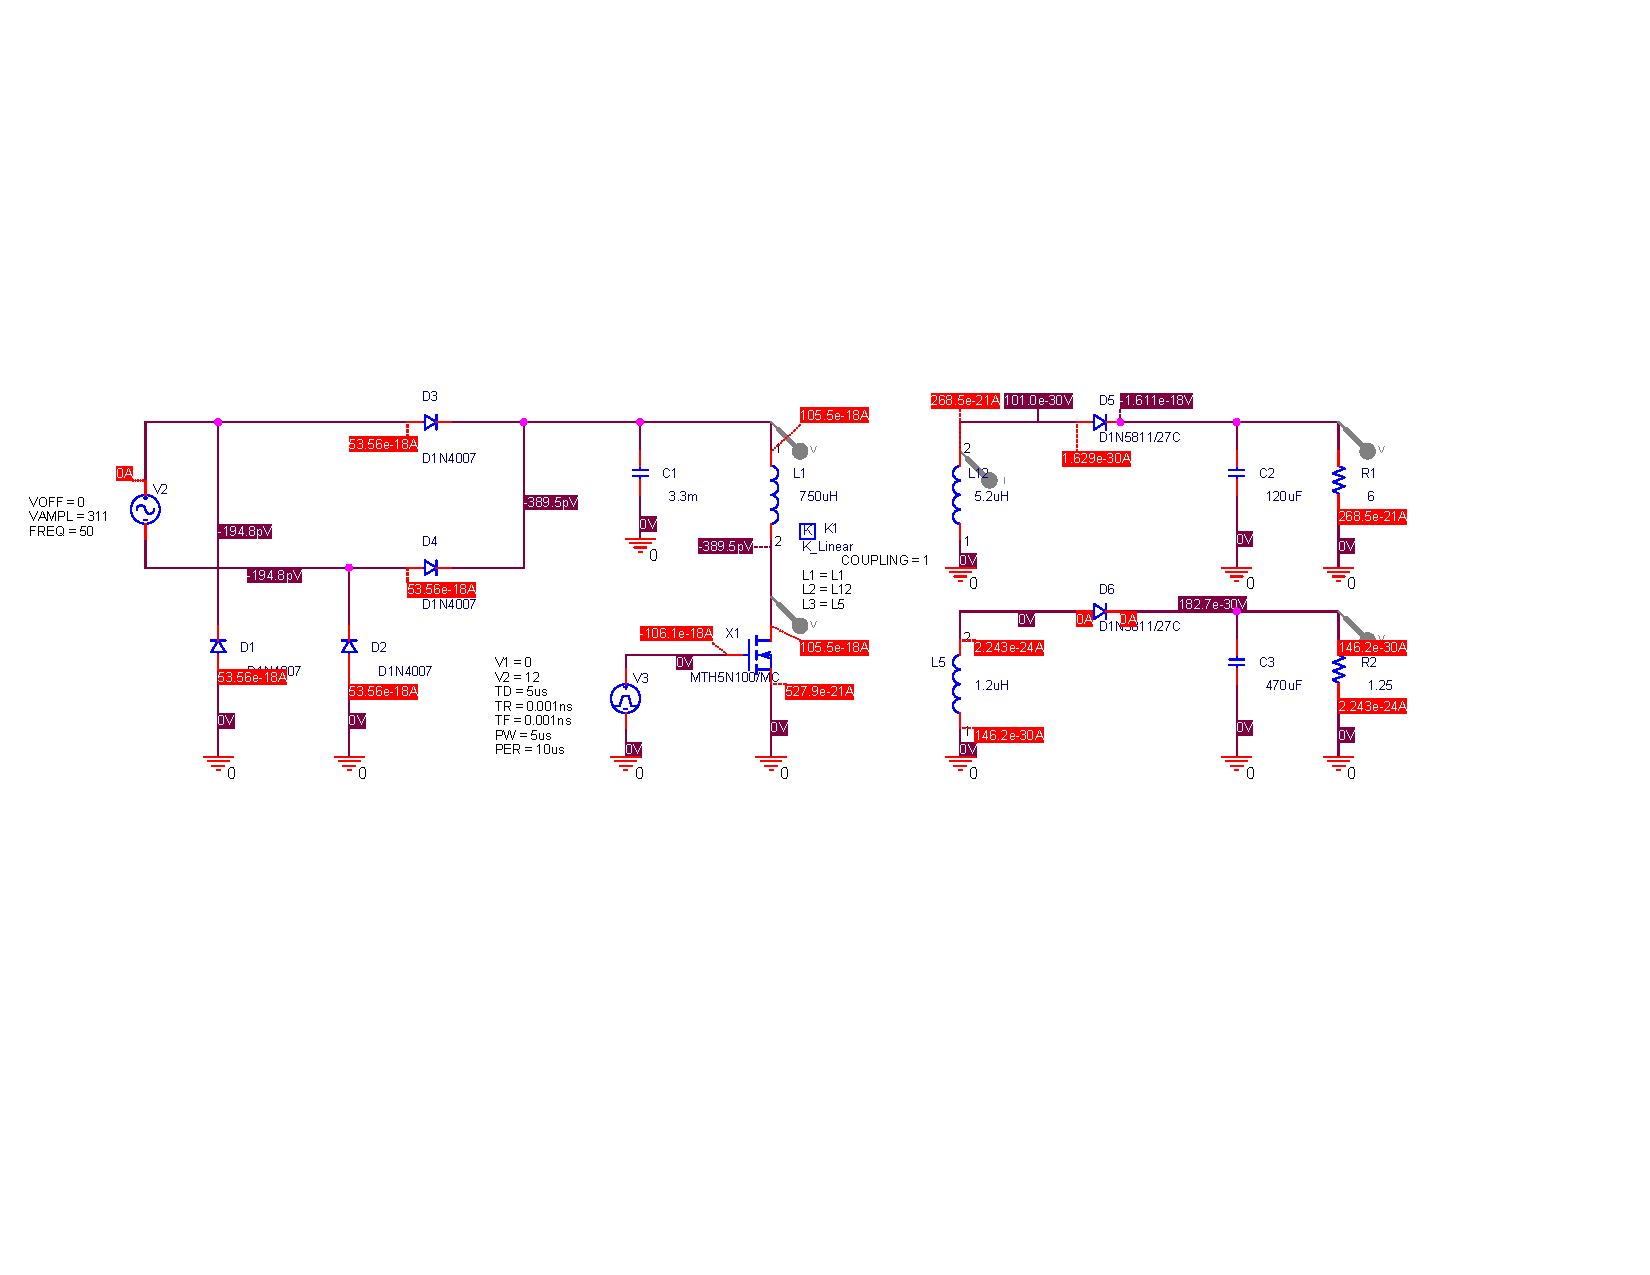
\includegraphics[scale=0.5]{Figuras/1_esquematico.pdf}
	\caption{Circuito bajo análisis con \textit{PSpice}.}
	\label{fig:esq}
\end{figure}


\Flor{Simulación hecha con $Vimax = \sqrt{2} 220V = 311V$. }
\begin{figure}[H]
	\centering
	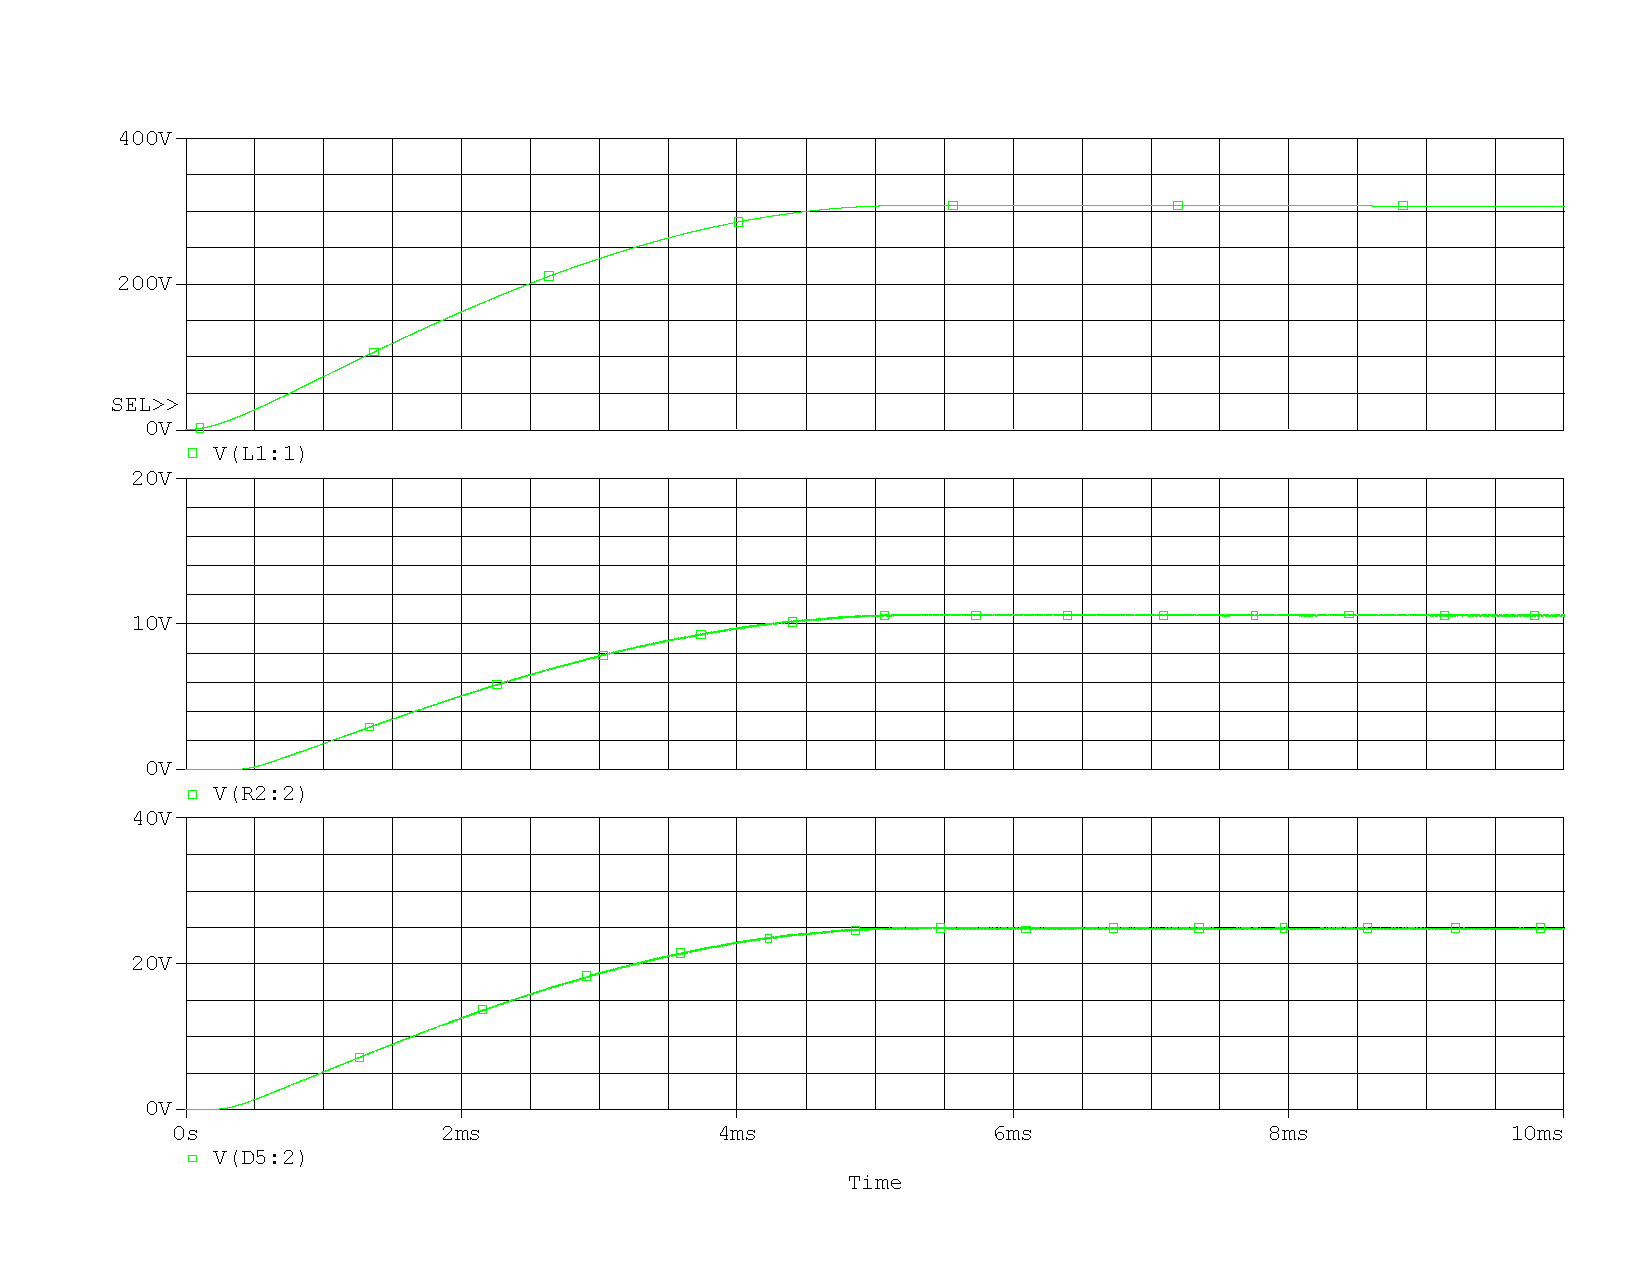
\includegraphics[scale=0.5]{Figuras/1_transitorio_con_rectificador.pdf}
	\caption{Transitorio.}
	\label{fig:transitorio}
\end{figure}

\begin{figure}[H]
	\centering
	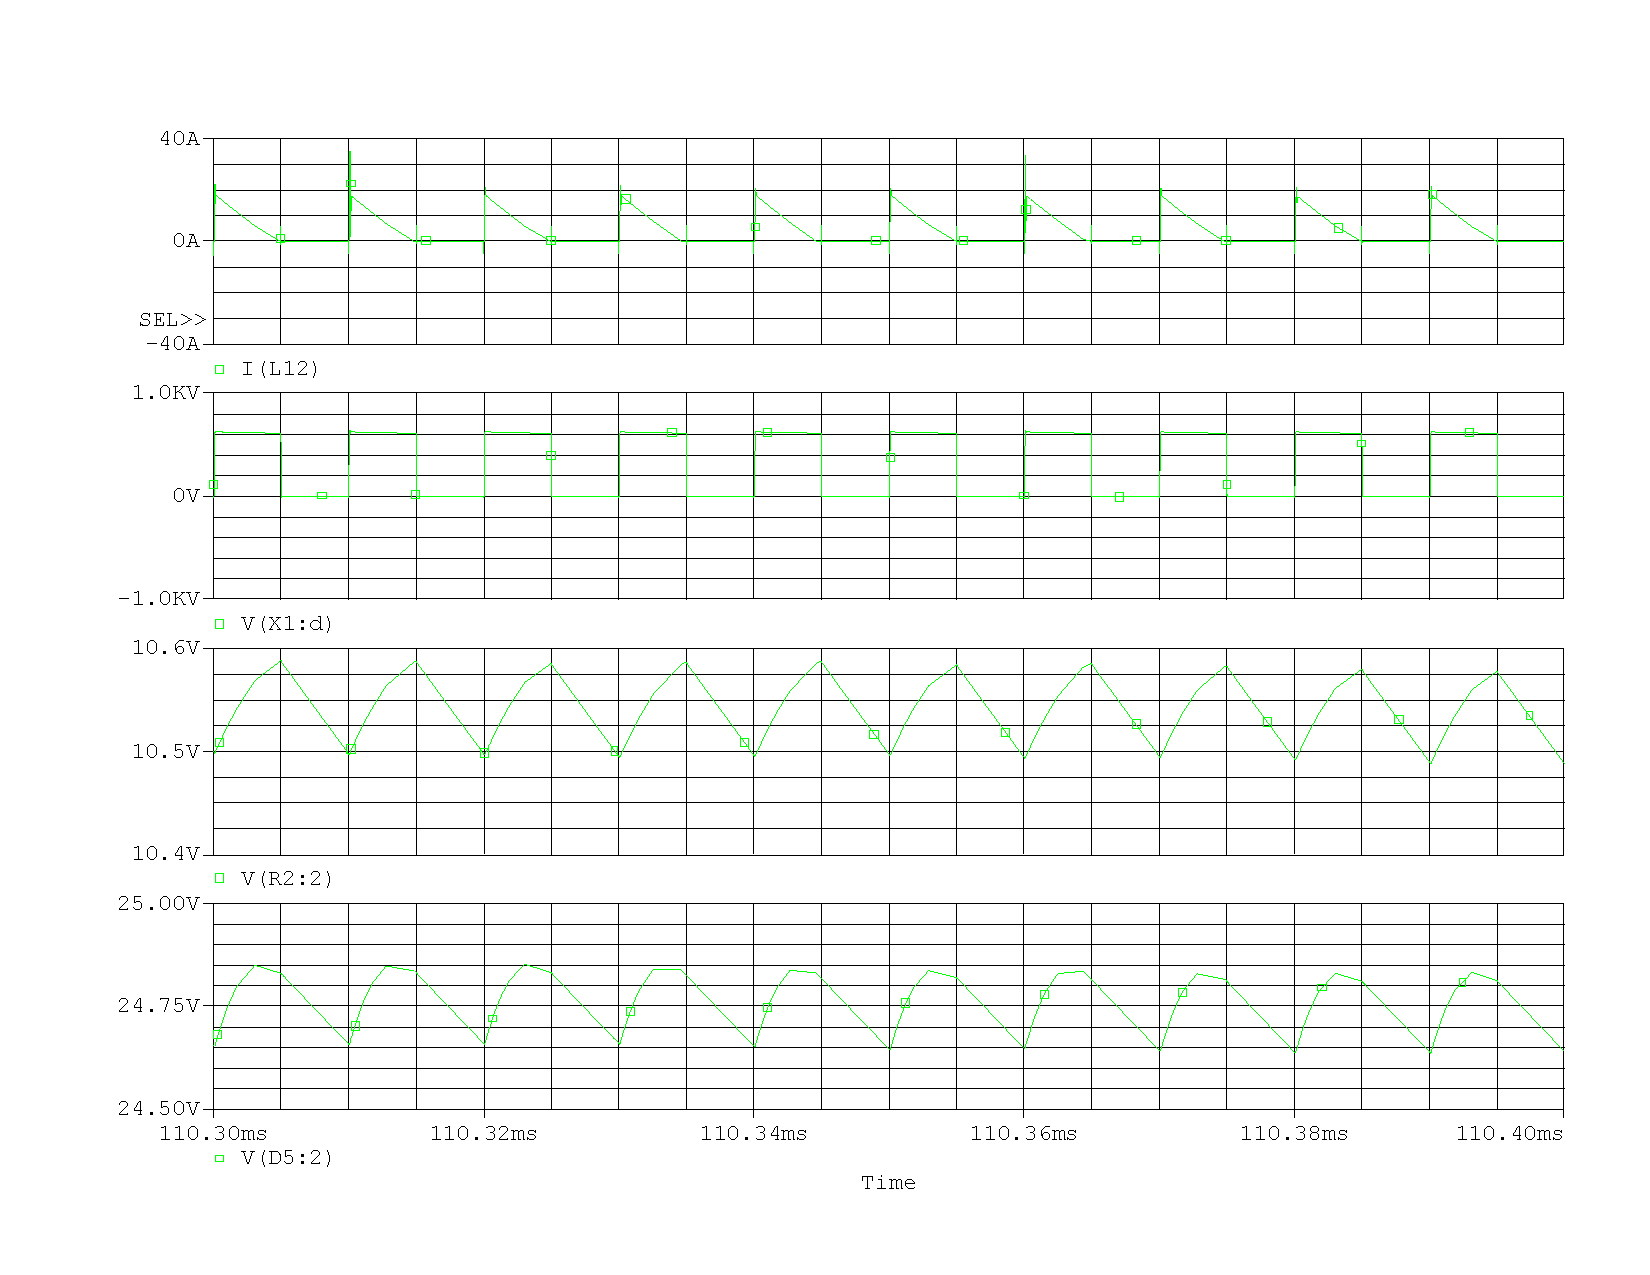
\includegraphics[scale=0.5]{Figuras/1_regimen_permanente.pdf}
	\caption{Régimen permanente.}
	\label{fig:permanente}
\end{figure}


